% REMEMBER: You must not plagiarise anything in your report. Be extremely careful.

\documentclass{l4proj}

    
% put any additional packages here
\usepackage{amsthm}
\usepackage{amssymb}
\usepackage{amsmath}
\usepackage{enumitem}


%==============================================================================
%% Commands 
\theoremstyle{definition}
\newtheorem{definition}{Definition}[section]

\setitemize{noitemsep}
%==============================================================================

\begin{document}

%==============================================================================
%% METADATA
\title{Recursive Paraphrasing on AI-Watermarked Text}
\author{Samuel Jackson}
\date{\today}

\maketitle

%==============================================================================
%% ABSTRACT
\begin{abstract}
    \textbf{Every abstract follows a similar pattern. Motivate; set aims; describe work; explain results.}
    \vskip 0.5em
    Given the rise of LLMs and the growing power of malicious content-generation, 
    methods of identifying and authenticating machine-generated content has become a necessity. 
    This paper aims to investigate the robustness of modern techniques in watermarking Transformer-based LLMs at inference through paraphrasing attacks. The paper presents evidence of poor defense towards paraphrasing attacks
    where even a simple paraphraser can reduce detect-ability by ??\%.
\end{abstract}

%==============================================================================

% EDUCATION REUSE CONSENT FORM
% If you consent to your project being shown to future students for educational purposes
% then insert your name and the date below to  sign the education use form that appears in the front of the document. 
% You must explicitly give consent if you wish to do so.
% If you sign, your project may be included in the Hall of Fame if it scores particularly highly.
%
% Please note that you are under no obligation to sign 
% this declaration, but doing so would help future students.
%
%\def\consentname {My Name} % your full name
%\def\consentdate {20 March 2018} % the date you agree
%
\educationalconsent


%==============================================================================
\tableofcontents

%==============================================================================
%% Notes on formatting
%==============================================================================
% The first page, abstract and table of contents are numbered using Roman numerals and are not
% included in the page count. 
%
% From now on pages are numbered
% using Arabic numerals. Therefore, immediately after the first call to \chapter we need the call
% \pagenumbering{arabic} and this should be called once only in the document. 
%
% Do not alter the bibliography style.
%
% The first Chapter should then be on page 1. You are allowed 40 pages for a 40 credit project and 30 pages for a 
% 20 credit report. This includes everything numbered in Arabic numerals (excluding front matter) up
% to but excluding the appendices and bibliography.
%
% You must not alter text size (it is currently 10pt) or alter margins or spacing.
%
%
%==================================================================================================================================
%
% IMPORTANT
% The chapter headings here are **suggestions**. You don't have to follow this model if
% it doesn't fit your project. Every project should have an introduction and conclusion,
% however. 
%
%==================================================================================================================================
\chapter{Introduction}

% reset page numbering. Don't remove this!
\pagenumbering{arabic} 


% This is straight bollocks. Pretend it does not exist.
Accredited to the rise of ChatGPT, we have seen Large Language Models (LLM) become mainstream alongside the text that they produce. The realistic appearance of unreliable text generated by these models fuels misinformation (reference), academic misconduct (reference) and fearmongering (reference). In an effort to help combat AI-generated text, methods of hiding digital signatures within text have been established, known as watermarks. 
\section{Guidance}

\textbf{Motivate} first, then state the general problem clearly. 

\section{Writing guidance}
\subsection{Who is the reader?}

This is the key question for any writing. Your reader:

\begin{itemize}
    \item
    is a trained computer scientist: \emph{don't explain basics}.
    \item
    has limited time: \emph{keep on topic}.
    \item
    has no idea why anyone would want to do this: \emph{motivate clearly}
    \item
    might not know \emph{anything} about your project in particular:
    \emph{explain your project}.
    \item
    but might know precise details and check them: \emph{be precise and
    strive for accuracy.}
    \item
    doesn't know or care about you: \emph{personal discussions are
    irrelevant}.
\end{itemize}

Remember, you will be marked by your supervisor and one or more members
of staff. You might also have your project read by a prize-awarding
committee or possibly a future employer. Bear that in mind.

\subsection{References and style guides}
There are many style guides on good English writing. You don't need to
read these, but they will improve how you write.

\begin{itemize}
    \item
    \emph{How to write a great research paper} \cite{Pey17} (\textbf{recommended}, even though you aren't writing a research paper)
    \item
    \emph{How to Write with Style} \cite{Von80}. Short and easy to read. Available online.
    \item
    \emph{Style: The Basics of Clarity and Grace} \cite{Wil09} A very popular modern English style guide.
    \item
    \emph{Politics and the English Language} \cite{Orw68}  A famous essay on effective, clear writing in English.
    \item
    \emph{The Elements of Style} \cite{StrWhi07} Outdated, and American, but a classic.
    \item
    \emph{The Sense of Style} \cite{Pin15} Excellent, though quite in-depth.
\end{itemize}

\subsubsection{Citation styles}

\begin{itemize}
\item If you are referring to a reference as a noun, then cite it as: ``\citet{Orw68} discusses the role of language in political thought.''
\item If you are referring implicitly to references, use: ``There are many good books on writing \citep{Orw68, Wil09, Pin15}.''
\end{itemize}

There is a complete guide on good citation practice by Peter Coxhead available here: \url{http://www.cs.bham.ac.uk/~pxc/refs/index.html}. 
If you are unsure about how to cite online sources, please see this guide: \url{https://student.unsw.edu.au/how-do-i-cite-electronic-sources}.

\subsection{Plagiarism warning}

\begin{highlight_title}{WARNING}
    
    If you include material from other sources without full and correct attribution, you are commiting plagiarism. The penalties for plagiarism are severe.
    Quote any included text and cite it correctly. Cite all images, figures, etc. clearly in the caption of the figure.
\end{highlight_title}


%==================================================================================================================================
\chapter{Background}
PROVIDE INTRO TO THIS BACKGROUND SECTION. 

\section{Textual Representation}
    In order to process text and train language models, we require datasets and numerical representations of text to provide our models and algorithms. These datasets are referred to as \emph{corpora}.

    A \emph{document} is an element of the corpus. % Better way to say this sentence
    To find the numerical representation of a document, irrelevant information is removed first through a process of known as tokenisation.
    \subsection{Tokenisation}
        \begin{definition}[Token]
            A \emph{token} is a sequence of characters, often referring to a word or a subword.
        \end{definition}

        % Perhaps I could reference how humans learn words from context instead.
        Often times, without noticing, the human brain overlooks words deemed unimportant \citep{Rayner2011-pk}. This phenomena is replicated within tokenisation as we aim to highlight important parts of document.

        Rule-based tokenisation exists in the form of lemmatization, stemming and stopword removal whereas tokenisation models are also developed through methods like training a Byte Pair Encoding (BPE) tokeniser \citep{Gage1994ANA, sennrich2016neural} on a text corpus.

        % Maybe another image of tokenisation but show different tokeniser. 
        \begin{figure}[h]
            \centering
            \includegraphics[width=1\linewidth]{images/background/tokenisation-process.png}
                \caption{Image portraying the tokenisation process. Tokenisation was completed using the \texttt{Mistral-7B-v0.1} tokeniser \citep{jiang2023mistral}, a BPE tokeniser.}
            \label{fig:tokenisation-process} 
        \end{figure}

        \begin{definition}[Vocabulary]
            A \emph{vocabulary} is the collection of tokens recognised by a tokenisation function.
        \end{definition}

        Importantly for our discussion on watermarking language models, the training of these tokenisation models generates a \emph{unique} vocabulary dependent on the text corpus. The tokenisation uniqueness is propagated through the transformer-based architecture into the embedding portion.

    \subsection{Embedding}
        Despite tokenisation providing a degree of structure to the unstructured data, the process of \emph{embedding} within a transformer-based architecture is crucial in allowing the model to identify semantic meaning and relationships between tokens. 

        Word embedding is a specialised form of principal component analysis (PCA), where we train a model to represent a token with reduced dimensions. This reduces dimensions as well as allows the model to gain insight into tokens.

        \begin{figure}[h]
            \centering
            \includegraphics[width=1\linewidth]{images/background/embedding-process.png}
                \caption{Preliminary image portraying the embedding process.}
            \label{fig:embedding-process} 
        \end{figure}

        I would like a descriptive image about this portion because it is certainly useful and somewhat difficult to understand. 
        
        Ask Jake about this. Show him my understanding through drawing.
        Hot Encoded Matrix is: [Context Window x Vocab Size]. Word Embedding Matrix is: [Vocab Size x Embedding Dimension]
        
        How does a decoder-only model have word embeddings?
        I am going to draw an image because it allows a simpler explanation at Maryland watermark stage.
        
\section{Generation}
    Causal language models, such as GPT2 \citep{gpt2Radford2019LanguageMAgpt}, use a decoder-only architecture, avoiding the encoding process. The encoder-lacking architecture is representative of the method of text generation within causal language models. 
    
    \subsection{Decoders}
        A causal model treats text generation as a predict-next-token task. The principle idea is to look at the previous tokens and consider which token is most likely to next appear. WE DON'T NEED AN ENCODER, BUT WHY?
    
        \begin{figure}[h]
            \centering
            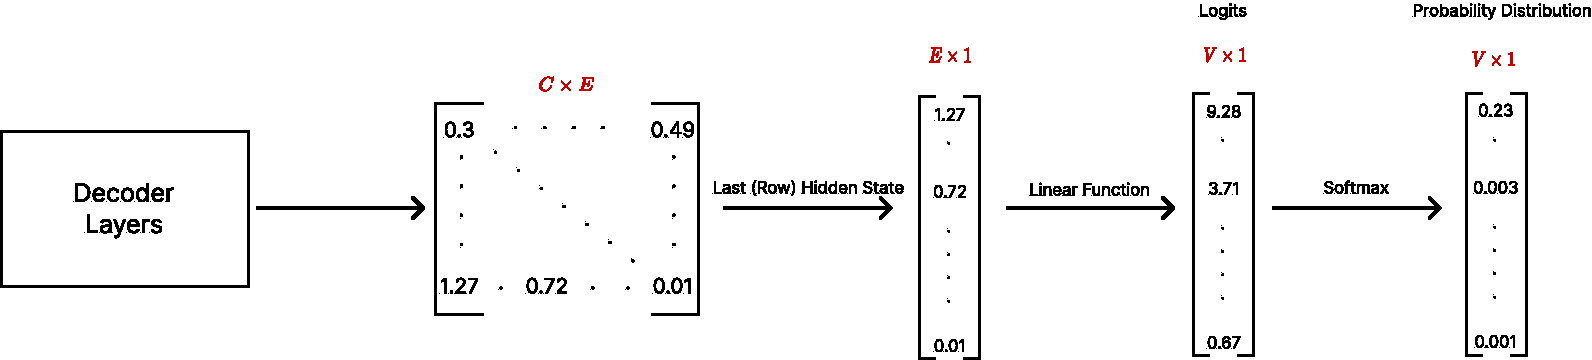
\includegraphics[width=1\linewidth]{images/background/decoding-process.png}
                \caption{Preliminary image portraying the decoding process.}
            \label{fig:embedding-process} 
        \end{figure}
    
        \begin{definition}[Logits]
            Let $p$ be the probability of an event happening. The \emph{logit}, or log odds of the event occurring is defined as: 
            \begin{align}
                \text{logit}(p) = \log\bigg(\frac{p}{1-p}\bigg),
            \end{align}
            where logit is defined as $\text{logit}: (0,1) \rightarrow (-\infty, \infty)$.
        \end{definition}
        
        The low probability values become negative under this method. This feature, alongside the wide range of values, provides simple interpretability. Hence, logits have become convention within language models.

    % This should probably be rewritten. 
    % Main points should be:
    %   - Large Language Models are intensive and trained differently.
    %   - Models have different broad architectures for different tasks.
    %   - Existing methods are an investigation on Causal Language Models.
    \subsection{Language Modelling}
        A Large Language Model (LLM) is an data-intensive machine learning model, expensively trained on large amounts of text. The training process will vary dependent on objective, and the architecture changes correspondingly.

        Models focused on translation, summarization and paraphrasing tend to be Sequence to Sequence (Seq2Seq) models. Seq2Seq models use an encoder-decoder architecture, encoding each token with reference to the entire input. The decoding is then completed in a left-to-right sequence.
`
        Famous services like ChatGPT are Causal Language models, using a unidirectional (left-to-right) decoder architecture. This means, at each stage, the generation of a token is only based on the previous tokens. 

% I like this section. Simply fill out photos and references now.
\section{Watermarks}
    \subsection{Content Watermarks}
        \begin{definition}[Watermark]
            A \emph{watermark} is a faint figure or signature designed to represent ownership or authorship.
        \end{definition}
        Watermarks can be found everywhere in every day life with examples ranging from the American 5 dollar bill to a music producer having an audio tag. 
        
        IMAGE EXAMPLE OF WATERMARK

        The varying methods of portraying media and art has required that methods of watermarking similarly grow in variety and effectiveness. \citet{xiang2017digital} covers traditional methods of audio watermarking, such as echo hiding and spread spectrum, which aim to achieve imperceptibility by deceiving our hearing. 
        
        PROVIDE METHODS OF IMAGE WATERMARKING 

        To hide a signature within text is a different task as it does not have the opportunity to deceive audio, whereas visual sensor could only be deceived through homoglyphs.
        Modern-day techniques use generative methods that allow for alterations in the text, be it the characters used or biasing particular tokens.
    \subsection{Text Watermark Requirements}
         Watermarks come in many forms, be it a signature: ``Written by Sam Jackson'' or a well-defined pattern of ending every word with the character `n'.
         
         Given the purpose of watermarking generative content, there are the following primary goals that an AI watermark aims to achieve:
         \begin{itemize}
            \setlength\itemsep{0.5em}
            \item \textbf{Robust} - Capable of withstanding attempts to remove watermark.
            \item \textbf{Agnostic} - Information beyond generated text is not required for detection.
            \item \textbf{Imperceptible} - The watermark should not be visible, be it a change in quality or a written signature.
        \end{itemize}
        These requirements are specifically designed to encourage watermarks which are zero-shot and capable of covering any generative large language model, even closed source models. \cite{perhaps an example/rewrite this}.
    \subsection{Attacking methods}
        No matter the robustness of a watermark, methods of successfully attacking are real threats. 

        A classic and simple technique is \emph{word-replacement}. This is a rule-based technique, free from computational constraints, which has success against models, as mentioned in \cite{reference here}, but suffers in textual clarity.

        Embedding generated-text within a larger document is a subtle method which can be successful. Students are known to have used AI for a particular paragraph or sentence of an essay, as opposed to the entire essay. Detection within a larger document is reported to be less successful \cite{okay okay, pray for the source} where only a small portion of the text is generated. 

        Opposing the prior methods, this method is particular to causal language modelling. Due to the nature of generative content, instructing the prompt can be an effective method to combat watermarking methods focused on manipulating the logits at inference time \citep{kirchenbauer2023watermark}. 

        One of the most intensive methods is paraphrasing. An advanced form of word-replacement that attempts to understand the underlying meaning of a text whilst re-structuring the text for their own purpose. This method is certainly the most computationally intensive as it requires a language model to re-structure the document, barring a rule-based paraphraser. The question that we discuss in this paper is whether the computational cost is worth it. 

\section{Paraphrasing}
    \subsection{English Definition \& Purpose}
        % I actually like this definition now.
        \begin{definition}[Paraphrase]
            To repeat something written or spoken using different words, often in a humorous form or in a simpler and shorter form that makes the original meaning clearer (Cambridge Dictionary, 2024).
        \end{definition}
    \subsection{Attacking Method}
        \begin{itemize}
            \setlength\itemsep{0.5em}
            \item Instead of altering generating content, the content is used as prompt.
            \item The model is funnelled through a Seq2Seq model (as opposed to causal), using an encoder-decoder architecture, to produce a paraphrase.
            \item By definition, defeats watermarkings methods like whitespacing and homoglyphs. 
        \end{itemize}
    \subsection{DIPPER Paraphrase Model}
        % Rewrite this paragraph.
        Paraphrasers are Seq2Seq models, as the task bears strong resemblance to translation. In fact, many models are trained on text which is twice-translated \citet{to french and back!}. Open-source paraphrasers fine-tuned on sentence translations (cite this?), leading to the sentence-context focus. Fortunately, there is one paper that generated their own paragraph-based paraphraser.

        % The twice-translation would be a simple photo, and interesting.
        % Perhaps I could evaluate with twice-translation too. 
    
        % Things that I want to mention
        %   - Paraphrase model developed in Retrieval paper. | TICK
        %   - Paraphraser has variable parameters, order and lexical diversity | TICK
        %   - Training completed through reordering paragraphs and aligning paragraphs from different translations. | TICK
        %   - Semantic similarity | TICK 
        
        Through the methods described in the paper by \citet{krishna2023paraphrasing}, a paraphraser which is focused on paragraph-context is developed. The paraphraser permits for variable amounts of change, with lexical diversity and sentence-order diversity as parameters are included in the paraphrasing process. 
        
        \citet{Par3_2022} provides a dataset of book translations, many of the same book. Through sentence realignment and order-shuffling, the model is fine-tuned on an artificial paragraph and scored against the original paragraph. Importantly, each document begins with variables for order and complexity. 

        % Maybe an image to describe this because it is not a simple concept.
    \subsection{Semantic Similarity}
        As defined earlier, paraphrasing is intended to maintain the original meaning. As a process, changing words and ordering of a document can impact the meaning. Hence, a similarity metric to consider differences numerically provides useful insight.

        Typically, we use the vector embeddings of documents to find the similarity through a given function. Mathematically, we define similarity as a function $\Omega : S \times S \rightarrow [0, 1]$. A popular such similarity measure is the cosine similarity function. 

        % TALK ABOUT FLAWS IN SIMILARITY MEASURE. 
        %   - Heavily dependent on context words (some words have greater bearing)
        %   - Larger document, each word has less meaning so harder to compare. 
        %   - Vector embeddings are a product of pre/fine-training so each model is different.

        % Continue writing about this
        % Be more precise in the differences, and why do they have to know this background? 
        Hence, we look towards a paraphrase similarity method proposed by \citet{wieting2023paraphrastic}. It maintains same similarity concepts but on a model which is focused on detecting paraphrase similarity.

\section{Literature Survey}
    \subsection{Maryland Watermark}
        Show pdf image which colours some parts green and some red, based on greenlist tokens.
        \begin{itemize}
            \setlength\itemsep{0.5em}
            \item Reference Kirchenbauer paper
            \item Discuss hard watermark method 
            \item Intro to soft watermark method
        \end{itemize}
    % \subsection{Stanford Distortion Method} % Is this even necessary? I don't think so.
    \subsection{Inevitability of Failed-Detections} % Rename 
        Talk about \citet{sadasivan2023aigenerated} and the statistical analysis deducing that detection methods will become obsolete.
    \subsection{Easy Watermarking Methods}
        Incredible paper about simple watermarks that covers the simple concepts. A brief section of the results portion prieves attacking methods to this technique \citep{sato2023embarrassingly}.

% This is just for me to remember. Not staying like this.
\section{Research Questions}
    Each section should have a reference to these questions in some way. i.e. How does this impact paraphrasing on a paragraph-level as opposed to sentence-based? 
    \subsection{Does recursive paraphrasing provide more effective removal of a watermark?}
    \subsection{How does sentence-based paraphrasing compare to paragraph-based paraphrasing?}
    \subsection{Is there feasibility of use within an academic context?}
    \subsection{Is a simple word replacement algorithm sufficient?}
    
    
%================================================================================================
\chapter{Methods}
\textbf{What did you do to implement this idea, and what technical achievements did you make?}

\section{Experimentation Approach}
    To show the robustness or fragility of the watermark, documents are generated with the watermark, using the soft method in \citet{kirchenbauer2023watermark}. The generated documents were consequently manipulated through various methods, such as paraphrasing and word-replacement. To understand the cost of attacking the documents, I use a document similarity measure as a way to determine how much of the original meaning is maintained.

    \begin{figure}[h]
        \centering
        \includegraphics[width=1\linewidth]{images/methods/flow-chart-method.pdf}
        \caption{Flow Chart describing the method of experimentation. NEEDS UPDATING}
        \label{fig:method-flow-chart} 
    \end{figure}

    The experimentation process is complete with an evaluation of Z-Scores, using a formula defined in \citet{kirchenbauer2023watermark}. The Z-Score permits a binary classification on whether the documents are watermarked, allowing us to identify the removal of a watermark. Furthermore, the multiple methods help us determine if paraphrasing is a necessary step in removing given watermark.

\section{Dataset}
    To generate our watermarked documents, an appropriate 
    \subsection{Source}
        From Kaggle, ongoing competition, aiming to detect AI Generated Text \citep{llm-detect-ai-generated-text}. The dataset provides real essays, scraped from a separate Kaggle competition \citet{link feedback prize 3 kaggle}.
        Give some more information on this. Are all prompts the same style? Are all prompts even tasks?
        
    \subsection{Other possible datasets}
        I chose to opt for a instruct model as opposed to an auto-generated method. The auto-generated method was experimented with, with a dataset from SignalMedia 1M Articles. 
    \subsection{Structure \& Sample}
        The dataset is composed of four columns: \textbf{id}, \textbf{text}, \textbf{instructions}, \textbf{source\_text}.

        TABLE DISPLAYING SAMPLE DOCUMENTS

\section{Model Selection}
    \subsection{Availability and Limitation}
        With access to 24GB VRAM, I had the opportunity to use models up to 7B models. Utilising methods like LoRA (Low-Rank Approximation) and half-precision (16-bit $\rightarrow$ 8-bit etc), I could use models up to 13B, sacrificing some accuracy. 
    \subsection{Prompt Generation}
        Talk about how I used instruct generation as opposed to autogenerated, as used in Maryland and Krishna (DIPPER).
    
\section{Implementation of Maryland Watermark}
    The Maryland Watermark \citep{kirchenbauer2023watermark} made the code publicly available, which aided in customising the method for my purposes.

    The implementation leverages the internals of HuggingFace and PyTorch. The figure \ref{fig:draw-this-figure} portrays the point at which changes are made. The post-training addition is a key selling point of the method, allowing for pre-existing models to adopt watermarking.

    % Think about what else to discuss here. Perhaps the delta and gamma scores? I fix these in my work so maybe reference as to why.

\section{Fine-tuning of a Paraphraser}
    The DIPPER paper \citep{krishna2023paraphrasing} provided the dataset, which is a processed version of the Par3 dataset \citep{Par3_2022}. Whilst the fine-tuned model was similarly available, the computational cost was too great. Hence, I fine-tuned a lower-cost variation.

    \subsection{Chosen Model}
        Respecting the initial paper, T5 was the chosen Seq2Seq model architecture for the paraphrasing task. The pretrained model was designed to investigate the potential of transfer-learning, hence lending itself to paraphrasing comfortably. 

        Within T5, numerous options are available. The paper, presented by \citet{tay2022scale}, provides analysis into efficient scaling as well as model checkpoints to be exploited. Amongst the efficient models, a DeepNarrow architecture is recommended to improve performance. This led to the decision to fine-tune the T5-Efficient-Large-NL32, where NL32 refers to the number of transformer blocks and Large refers to the approximately 1 billion parameters.

    \subsection{Training Approach}
        The initial paper fine-tuned their model on $\sim$6,000,000 paraphrase pairs, taking between 384 and 768 GPU hours \citep{krishna2023paraphrasing}. Incapable of replicating the same compute periods, the model I produced was fine-tuned on 100,000 paraphrase pairs, taking 12 GPU hours.
        Further specifications into the training arguments are in the appendix. % Refer to appendix.

        The dataset provided by DIPPER is split between Google translated and human translated. These sections are further split into nondescript subsections. In an effort to replicate the original paper to the fullest, both sections were sampled, taking a uniform distribution of documents from the respective subsections. 
        The dataset used is now publicly available.
        
\section{Generating Results} % Name this something better
    The watermark can only be applied at inference stage, hence the data generation process required to begin with creating watermarked documents. 

    \subsection{Watermarking Documents}
        How did this process function? Provided a prompt, the chosen model would generate two essays, watermarked and unwatermarked. The generation was nucleus-sampling (should make it nucleus sampling) with $p = 0.8$ (give reasons for this?) \newline 

    \subsection{Paraphrasing Documents}
        This was a two pronged approach. Paraphrasing had to be completed many times, over many documents. Perhaps I could have used some distributed processing for this portion. 
        I had to paraphrase with a sentence-based paraphraser as well as a paragraph-based.

    \subsection{Evaluating Documents}
        Respecting the initial threshold proposed by \citet{kirchenbauer2023watermark}, the Z-Score threshold was $z = 4.0$, based on the gamma and delta previously fixed ($\delta = 5.0, \gamma = 0.25$). 

% \section{General points}
% These points apply to the whole dissertation, not just this chapter.

% FIGURES --------------------------------------------------------
% \subsection{Figures}
% \emph{Always} refer to figures included, like Figure \ref{fig:relu}, in the body of the text. Include full, explanatory captions and make sure the figures look good on the page.
% You may include multiple figures in one float, as in Figure \ref{fig:synthetic}, using \texttt{subcaption}, which is enabled in the template.



% Figures are important. Use them well.
% \begin{figure}
%     \centering
%     \includegraphics[width=0.5\linewidth]{images/relu.pdf}    

%     \caption{In figure captions, explain what the reader is looking at: ``A schematic of the rectifying linear unit, where $a$ is the output amplitude,
%     $d$ is a configurable dead-zone, and $Z_j$ is the input signal'', as well as why the reader is looking at this: 
%     ``It is notable that there is no activation \emph{at all} below 0, which explains our initial results.'' 
%     \textbf{Use vector image formats (.pdf) where possible}. Size figures appropriately, and do not make them over-large or too small to read.
%     }

%     % use the notation fig:name to cross reference a figure
%     \label{fig:relu} 
% \end{figure}

% \begin{figure}
%     \centering
%     \begin{subfigure}[b]{0.45\textwidth}
%         \includegraphics[width=\textwidth]{images/synthetic.png}
%         \caption{Synthetic image, black on white.}
%         \label{fig:syn1}
%     \end{subfigure}
%     ~ %add desired spacing between images, e. g. ~, \quad, \qquad, \hfill etc. 
%       %(or a blank line to force the subfigure onto a new line)
%     \begin{subfigure}[b]{0.45\textwidth}
%         \includegraphics[width=\textwidth]{images/synthetic_2.png}
%         \caption{Synthetic image, white on black.}
%         \label{fig:syn2}
%     \end{subfigure}
%     ~ %add desired spacing between images, e. g. ~, \quad, \qquad, \hfill etc. 
%     %(or a blank line to force the subfigure onto a new line)    
%     \caption{Synthetic test images for edge detection algorithms. \subref{fig:syn1} shows various gray levels that require an adaptive algorithm. \subref{fig:syn2}
%     shows more challenging edge detection tests that have crossing lines. Fusing these into full segments typically requires algorithms like the Hough transform.
%     This is an example of using subfigures, with \texttt{subref}s in the caption.
%     }\label{fig:synthetic}
% \end{figure}

% \clearpage

% EQUATIONS --------------------------------------------------------
% \subsection{Equations}

% Equations should be typeset correctly and precisely. Make sure you get parenthesis sizing correct, and punctuate equations correctly 
% (the comma is important and goes \emph{inside} the equation block). Explain any symbols used clearly if not defined earlier. 

% For example, we might define:
% \begin{equation}
%     \hat{f}(\xi) = \frac{1}{2}\left[ \int_{-\infty}^{\infty} f(x) e^{2\pi i x \xi} \right],
% \end{equation}    
% where $\hat{f}(\xi)$ is the Fourier transform of the time domain signal $f(x)$.

% ALGORITHMS --------------------------------------------------------
% \subsection{Algorithms}
% Algorithms can be set using \texttt{algorithm2e}, as in Algorithm \ref{alg:metropolis}.

% % NOTE: line ends are denoted by \; in algorithm2e
% \begin{algorithm}
%     \DontPrintSemicolon
%     \KwData{$f_X(x)$, a probability density function returing the density at $x$.\; $\sigma$ a standard deviation specifying the spread of the proposal distribution.\;
%     $x_0$, an initial starting condition.}
%     \KwResult{$s=[x_1, x_2, \dots, x_n]$, $n$ samples approximately drawn from a distribution with PDF $f_X(x)$.}
%     \Begin{
%         $s \longleftarrow []$\;
%         $p \longleftarrow f_X(x)$\;
%         $i \longleftarrow 0$\;
%         \While{$i < n$}
%         {
%             $x^\prime \longleftarrow \mathcal{N}(x, \sigma^2)$\;
%             $p^\prime \longleftarrow f_X(x^\prime)$\;
%             $a \longleftarrow \frac{p^\prime}{p}$\;
%             $r \longleftarrow U(0,1)$\;
%             \If{$r<a$}
%             {
%                 $x \longleftarrow x^\prime$\;
%                 $p \longleftarrow f_X(x)$\;
%                 $i \longleftarrow i+1$\;
%                 append $x$ to $s$\;
%             }
%         }
%     }
    
% \caption{The Metropolis-Hastings MCMC algorithm for drawing samples from arbitrary probability distributions, 
% specialised for normal proposal distributions $q(x^\prime|x) = \mathcal{N}(x, \sigma^2)$. The symmetry of the normal distribution means the acceptance rule takes the simplified form.}\label{alg:metropolis}
% \end{algorithm}

% PSEUDOCODE RULES --------------------------------------------------------
% \begin{table}[]
%     \caption{The standard table of operators in Python, along with their functional equivalents from the \texttt{operator} package. Note that table
%     captions go above the table, not below. Do not add additional rules/lines to tables. }\label{tab:operators}
%     %\tt 
%     \rowcolors{2}{}{gray!3}
%     \begin{tabular}{@{}lll@{}}
%     %\toprule
%     \textbf{Operation}    & \textbf{Syntax}                & \textbf{Function}                            \\ %\midrule % optional rule for header
%     Addition              & \texttt{a + b}                          & \texttt{add(a, b)}                                    \\
%     Concatenation         & \texttt{seq1 + seq2}                    & \texttt{concat(seq1, seq2)}                           \\
%     Containment Test      & \texttt{obj in seq}                     & \texttt{contains(seq, obj)}                           \\
%     Division              & \texttt{a / b}                          & \texttt{div(a, b) }  \\
%     Division              & \texttt{a / b}                          & \texttt{truediv(a, b) } \\
%     Division              & \texttt{a // b}                         & \texttt{floordiv(a, b)}                               \\
%     Bitwise And           & \texttt{a \& b}                         & \texttt{and\_(a, b)}                                  \\
%     Bitwise Exclusive Or  & \texttt{a \textasciicircum b}           & \texttt{xor(a, b)}                                    \\
%     Bitwise Inversion     & \texttt{$\sim$a}                        & \texttt{invert(a)}                                    \\
%     Bitwise Or            & \texttt{a | b}                          & \texttt{or\_(a, b)}                                   \\
%     Exponentiation        & \texttt{a ** b}                         & \texttt{pow(a, b)}                                    \\
%     Identity              & \texttt{a is b}                         & \texttt{is\_(a, b)}                                   \\
%     Identity              & \texttt{a is not b}                     & \texttt{is\_not(a, b)}                                \\
%     Indexed Assignment    & \texttt{obj{[}k{]} = v}                 & \texttt{setitem(obj, k, v)}                           \\
%     Indexed Deletion      & \texttt{del obj{[}k{]}}                 & \texttt{delitem(obj, k)}                              \\
%     Indexing              & \texttt{obj{[}k{]}}                     & \texttt{getitem(obj, k)}                              \\
%     Left Shift            & \texttt{a \textless{}\textless b}       & \texttt{lshift(a, b)}                                 \\
%     Modulo                & \texttt{a \% b}                         & \texttt{mod(a, b)}                                    \\
%     Multiplication        & \texttt{a * b}                          & \texttt{mul(a, b)}                                    \\
%     Negation (Arithmetic) & \texttt{- a}                            & \texttt{neg(a)}                                       \\
%     Negation (Logical)    & \texttt{not a}                          & \texttt{not\_(a)}                                     \\
%     Positive              & \texttt{+ a}                            & \texttt{pos(a)}                                       \\
%     Right Shift           & \texttt{a \textgreater{}\textgreater b} & \texttt{rshift(a, b)}                                 \\
%     Sequence Repetition   & \texttt{seq * i}                        & \texttt{repeat(seq, i)}                               \\
%     Slice Assignment      & \texttt{seq{[}i:j{]} = values}          & \texttt{setitem(seq, slice(i, j), values)}            \\
%     Slice Deletion        & \texttt{del seq{[}i:j{]}}               & \texttt{delitem(seq, slice(i, j))}                    \\
%     Slicing               & \texttt{seq{[}i:j{]}}                   & \texttt{getitem(seq, slice(i, j))}                    \\
%     String Formatting     & \texttt{s \% obj}                       & \texttt{mod(s, obj)}                                  \\
%     Subtraction           & \texttt{a - b}                          & \texttt{sub(a, b)}                                    \\
%     Truth Test            & \texttt{obj}                            & \texttt{truth(obj)}                                   \\
%     Ordering              & \texttt{a \textless b}                  & \texttt{lt(a, b)}                                     \\
%     Ordering              & \texttt{a \textless{}= b}               & \texttt{le(a, b)}                                     \\
%     % \bottomrule
%     \end{tabular}
%     \end{table}
% \subsection{Code}

Avoid putting large blocks of code in the report (more than a page in one block, for example). Use syntax highlighting if possible, as in Listing \ref{lst:callahan}.

%==================================================================================================================================
\chapter{Results} 
\textbf{How good is your solution? How well did you solve the general problem, and what evidence do you have to support that?}

\section{Recursive Paragraph-Paraphrasing}
    \subsection{Graph}
        Goal is portray the effectiveness of paraphrasing to Z-Score whilst portraying the insignificance of repeatedly paraphrasing.

        Effectiveness of paraphrasing could be portrayed through scatterplot, drastically reducing Z-Score. \newline 

        In terms of evaluation, do we evaluate all generated documents? What if the document is less than 16 tokens? That is statistically the minimum required to detect a watermark from Maryland at $z = 4$.
    \subsection{Convergence of Results}
    \subsection{Semantic Similarity}
        Use Weiting PS-P for paraphrase similarity measure. \citep{wieting2021paraphrastic}
\section{Paragraph-based vs Sentence-Based}
    \subsection{Graph}
        Goal is to show that both sentence-based and paragraph-based techniques work. The tradeoff between techniques lies in the quality of paraphrases.

        Subplots of scatterplots will show effectivness and similarities.
        Need a way to show differing paraphrase-similarity scores.
    \subsection{Confusion Matrix discussion}
        Evaluation to table of tpr and fpr. Varying independent factor will be ??
\section{Word Replacement Insufficiency}
    
    \subsection{Graph}
        Graph displaying the lack of change within the Z-Score
        Could comfortably make an evaluation which varies the percentage of words replaced.

        Would expect word replacement to be effective when word-replacement \% > $\gamma$. 
    \subsection{Robustness of Method}
        Explanation for why the watermarking method remains robust.
\section{Feasibility of use in Academic Context}
    \subsection{Reasonable Cost of Paraphrase Use}
        Computational cost of methods presented.
    \subsection{Alternative Methods}
        At the cost of these methods, seems reasonable to use these methods. However, online website already provide these services - at a monetary cost as opposed to computational. Methods like prompt engineering are very real, as mentioned in \citet{kirchenbauer2023watermark}.

If you visualise, follow the basic rules, as illustrated in Figure \ref{fig:boxplot}:
\begin{itemize}
\item Label everything correctly (axis, title, units).
\item Caption thoroughly.
\item Reference in text.
\item \textbf{Include appropriate display of uncertainty (e.g. error bars, Box plot)}
\item Minimize clutter.
\end{itemize}

See the file \texttt{guide\_to\_visualising.pdf} for further information and guidance.

% \begin{figure}
%     \centering
%     \includegraphics[width=1.0\linewidth]{images/boxplot_finger_distance.pdf}    

%     \caption{Average number of fingers detected by the touch sensor at different heights above the surface, averaged over all gestures. Dashed lines indicate
%     the true number of fingers present. The Box plots include bootstrapped uncertainty notches for the median. It is clear that the device is biased toward 
%     undercounting fingers, particularly at higher $z$ distances.
%     }

%     % use the notation fig:name to cross reference a figure
%     \label{fig:boxplot} 
% \end{figure}


%==================================================================================================================================

% \chapter{Related Work}
% Background will discuss relevant information to understand this project. Related work will discuss other approaches to the topic.

% Maybe mention generative text like code - this cannot be effectively paraphrased.

%==================================================================================================================================
\chapter{Conclusion}    
Summarise the whole project for a lazy reader who didn't read the rest (e.g. a prize-awarding committee).
\section{Guidance}
\begin{itemize}
    \item
        Summarise briefly and fairly.
    \item
        You should be addressing the general problem you introduced in the
        Introduction.        
    \item
        Include summary of concrete results (``the new compiler ran 2x
        faster'')
    \item
        Indicate what future work could be done, but remember: \textbf{you
        won't get credit for things you haven't done}.
\end{itemize}

\section{Limitations}
\section{Future Work}
\section{Personal Thoughts}

%====== ============================================================================================================================
%
% 
%==================================================================================================================================
%  APPENDICES  

\begin{appendices}

\chapter{Appendices}

Typical inclusions in the appendices are:

\begin{itemize}
\item
  Copies of ethics approvals (required if obtained)
\item
  Copies of questionnaires etc. used to gather data from subjects.
\item
  Extensive tables or figures that are too bulky to fit in the main body of
  the report, particularly ones that are repetitive and summarised in the body.

\item Outline of the source code (e.g. directory structure), or other architecture documentation like class diagrams.

\item User manuals, and any guides to starting/running the software.

\end{itemize}

\textbf{Don't include your source code in the appendices}. It will be
submitted separately.

\end{appendices}

%==================================================================================================================================
%   BIBLIOGRAPHY   

% The bibliography style is abbrvnat
% The bibliography always appears last, after the appendices.

\bibliographystyle{abbrvnat}

\bibliography{l4proj}

\end{document}
